\section{Precession Raw Data} \label{sec:appendix:precession_raw_data}
In figure \ref{fig:appendix:raw_precession_data}, eleven measurements for precession frequency for different torques and initial spinning angular velocities ($\boldsymbol\omega_{3}$) are depicted with their mean values.

Because of the reasons discussed in section TODO, measurements $2, 8$ and $10$ have unique torque-$\boldsymbol\omega_3$ combinations. Thus, they do not have a pair of measurements to calculate the mean squared error for their unique torque-$\boldsymbol\omega_3$ combinations (see appendix \ref{appendix:errors} for error analysis)\footnote{However, their error was estimated by the standard error elicited from their time distribution.}. Consequently, they are referred to as \emph{Type I} measurements in figure \ref{fig:results:processed_precession}.

In contrast, all other measurements have a pair\footnote{That is, these pairs of measurements have the same torque-$\boldsymbol\omega_3$ combination.}, including $\#1 (4/5)$, $\#2 (3/7)$, $\#3 (1/9)$, $\#4 (6/11)$ points. In figure \ref{fig:results:processed_precession}, they are referred to as \emph{Type II} measurements.

\begin{figure}[!ht]
  \centering
  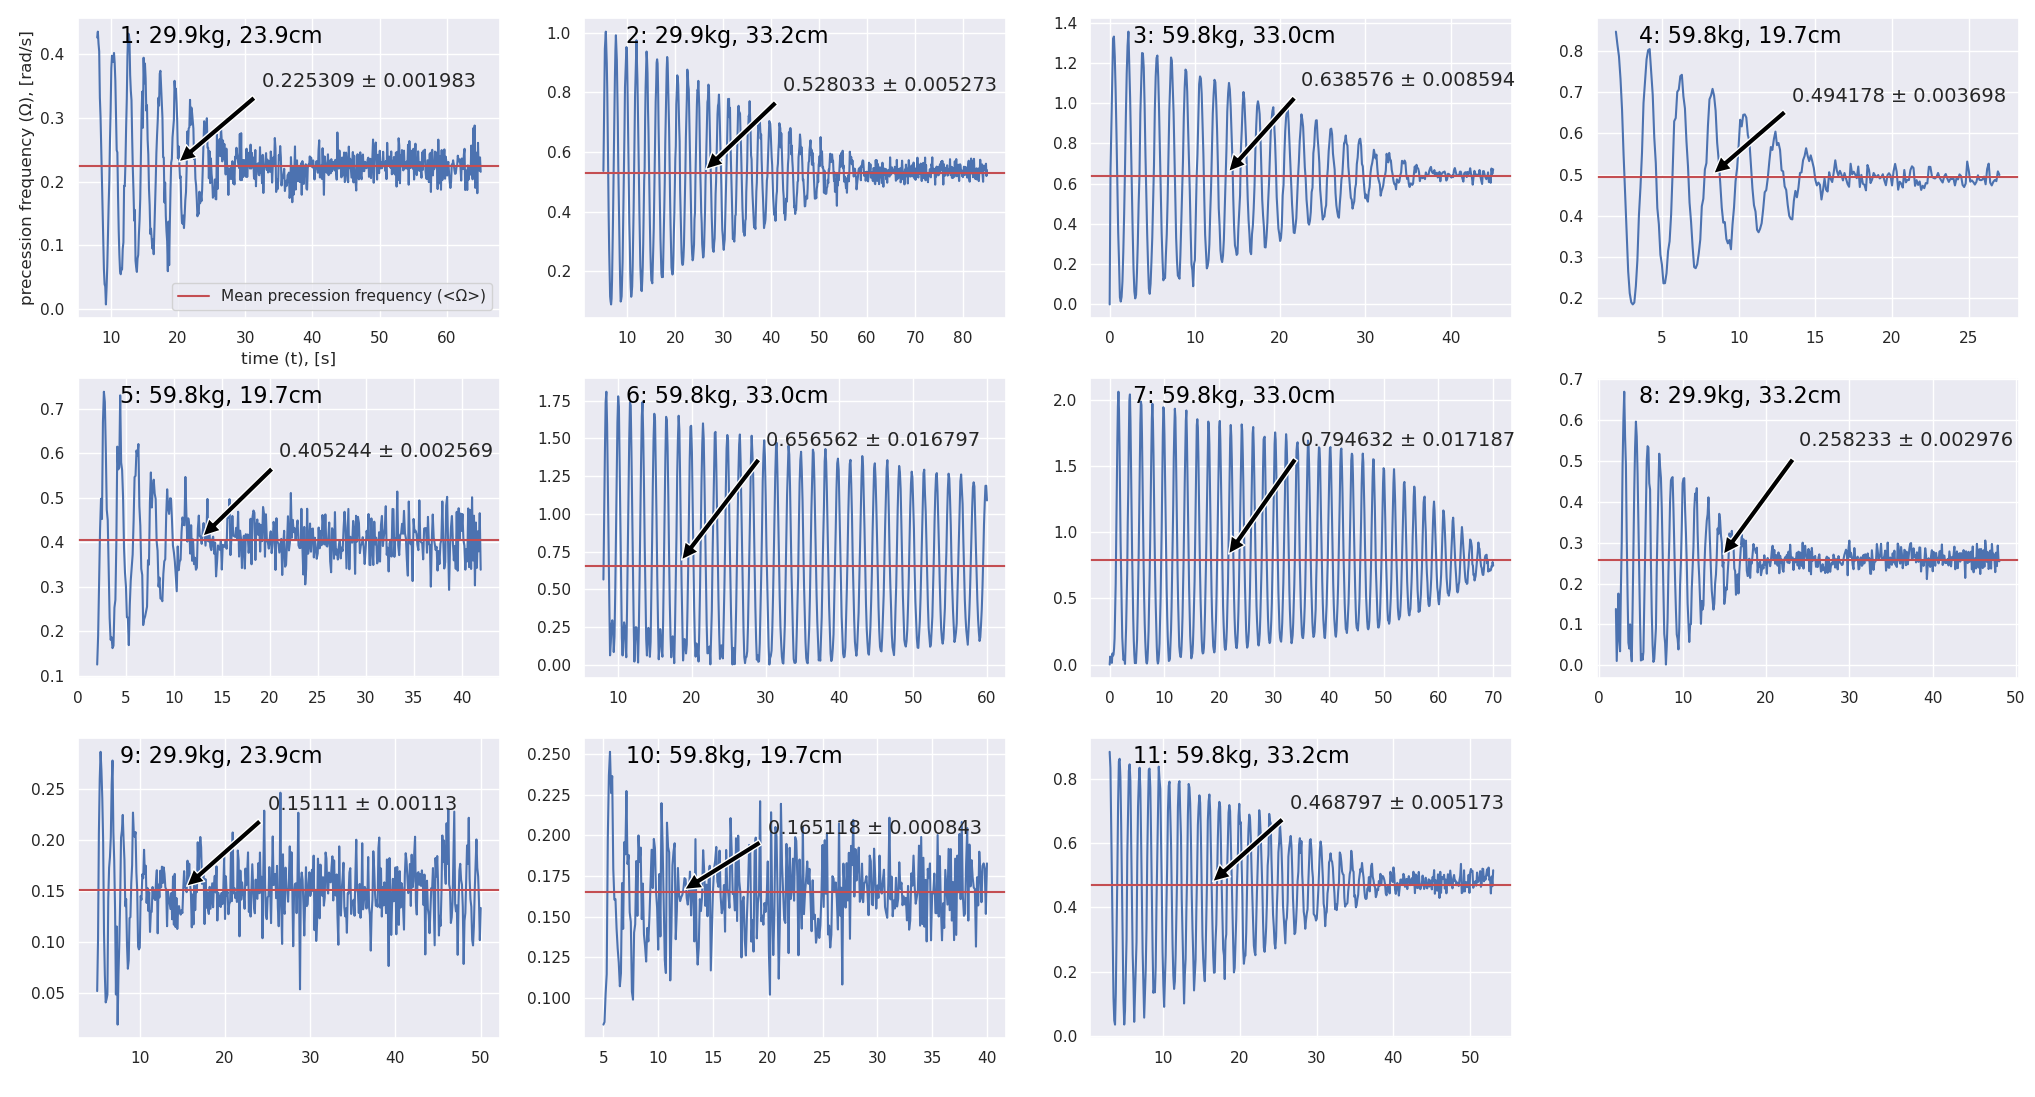
\includegraphics[width=\textwidth]{gyroscope/images/raw_precession}
  \caption{Raw precession frequency data from TISensorTag, and mean values}
  \label{fig:appendix:raw_precession_data}
\end{figure}

\begin{figure}[!ht]
  \centering
  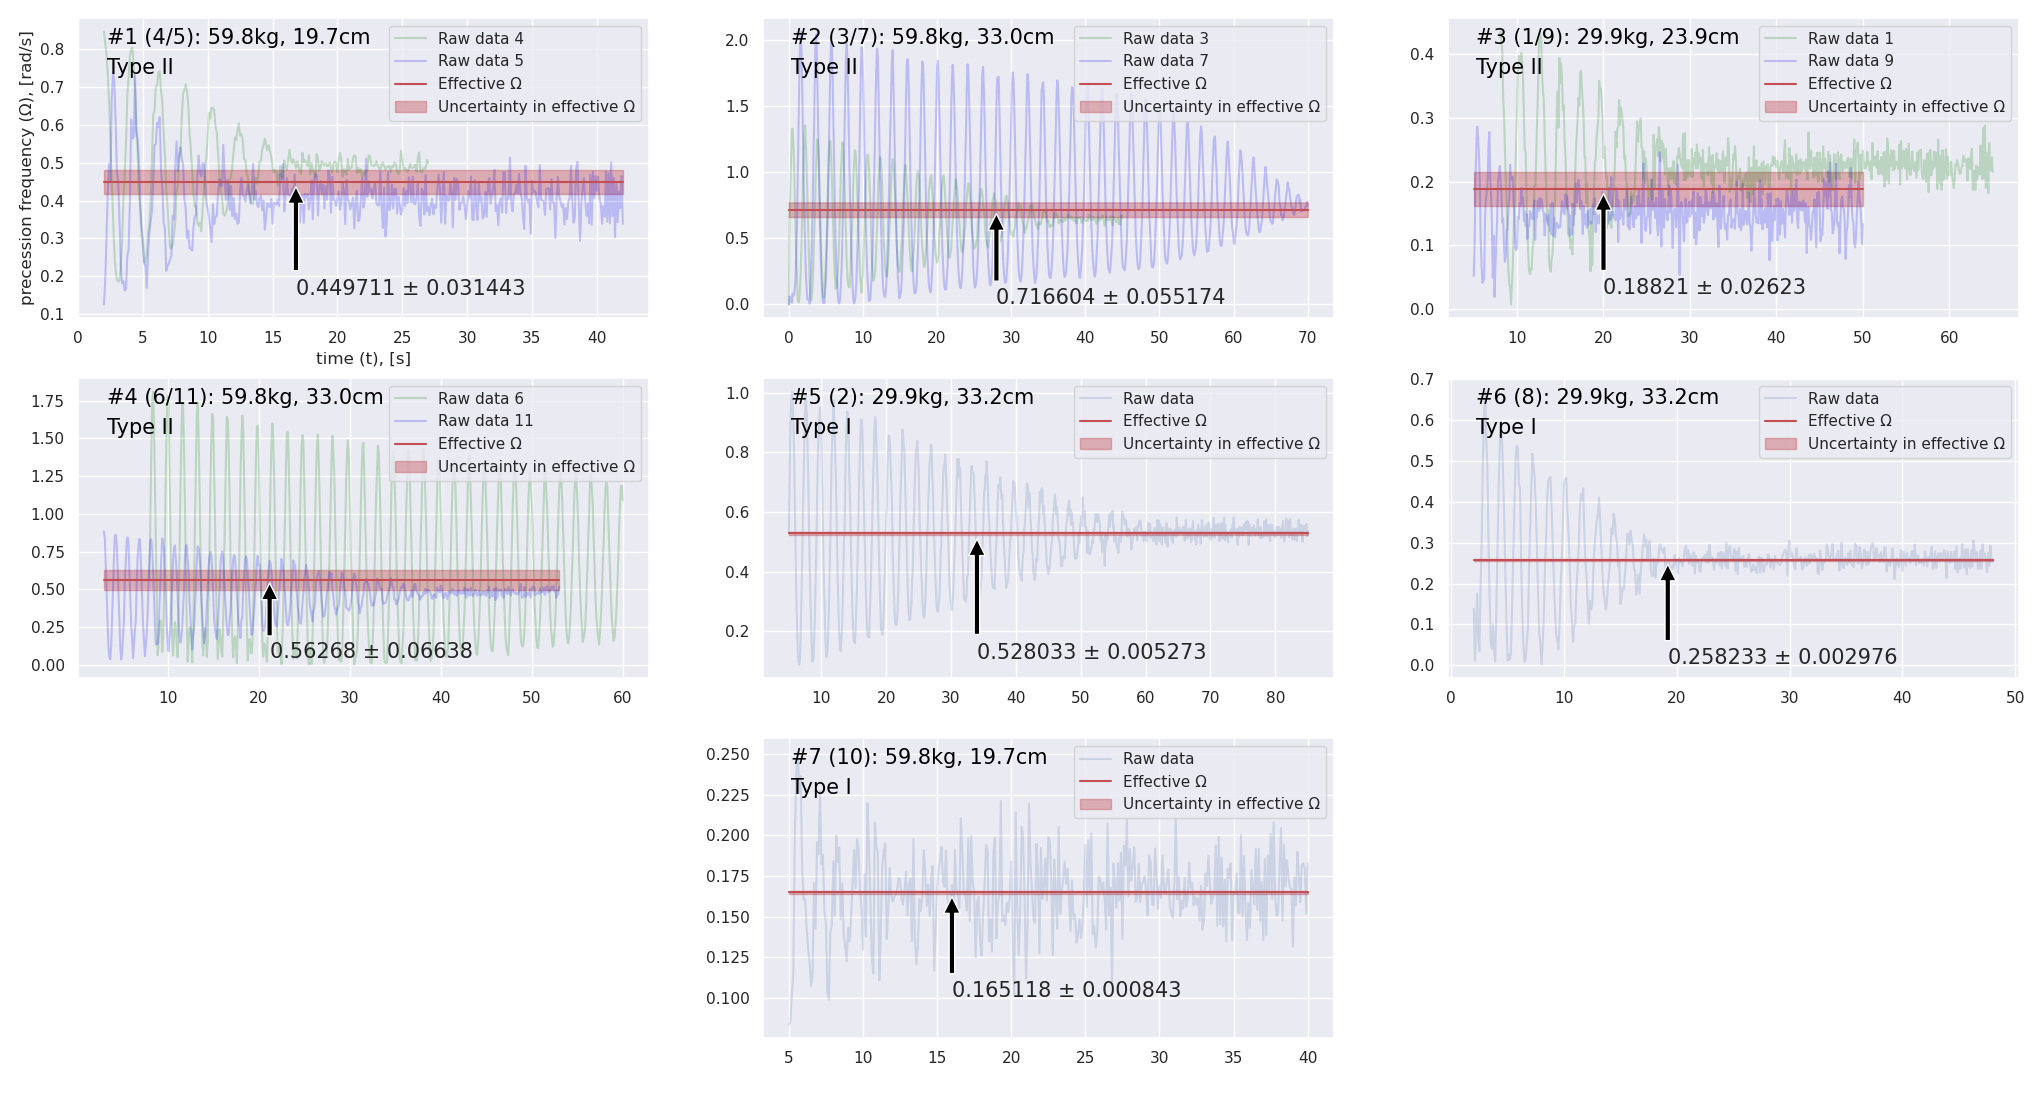
\includegraphics[width=\textwidth]{gyroscope/images/processed_precession}
  \caption{Processed precession frequencies ($\Omega$) }  
  \label{fig:results:processed_precession}
\end{figure}

Table TODO in section \ref{sec:results} contains effective precession frequencies and their uncertainties for each torque-$\boldsymbol\omega_{3}$ combination depicted by the solid red line in figure \ref{fig:results:processed_precession}.
